% !TeX root = ../main.tex
% Add the above to each chapter to make compiling the PDF easier in some editors.

\chapter{Implementation}\label{chapter:implementation}
We now turn to the implementation of our prototype live streaming system. We first give a high-level overview of the architecture, and then we proceed with discussing in more depth the inner workings of the client and the server. We will describe the concrete streaming protocols in later sections. Our prototype uses draft version 3 of \ac{MOQT}, but the main points outlined in this section should be applicable to later versions as well.

The architecture of our prototype live streaming system can be seen in \autoref{fig:architecture}. The origin server ingests a live video stream through stdin and broadcasts it to clients using \ac{MoQ}. The video stream is transmitted directly from the origin server to clients without passing to relays. The live video stream is produced with FFmpeg\footnote{\url{https://www.ffmpeg.org/}}, which reads a source video at the native frame rate to simulate live streaming. We reencode the source video with H.264/AVC and package it in MP4 fragments.

\begin{figure}
    \centering
    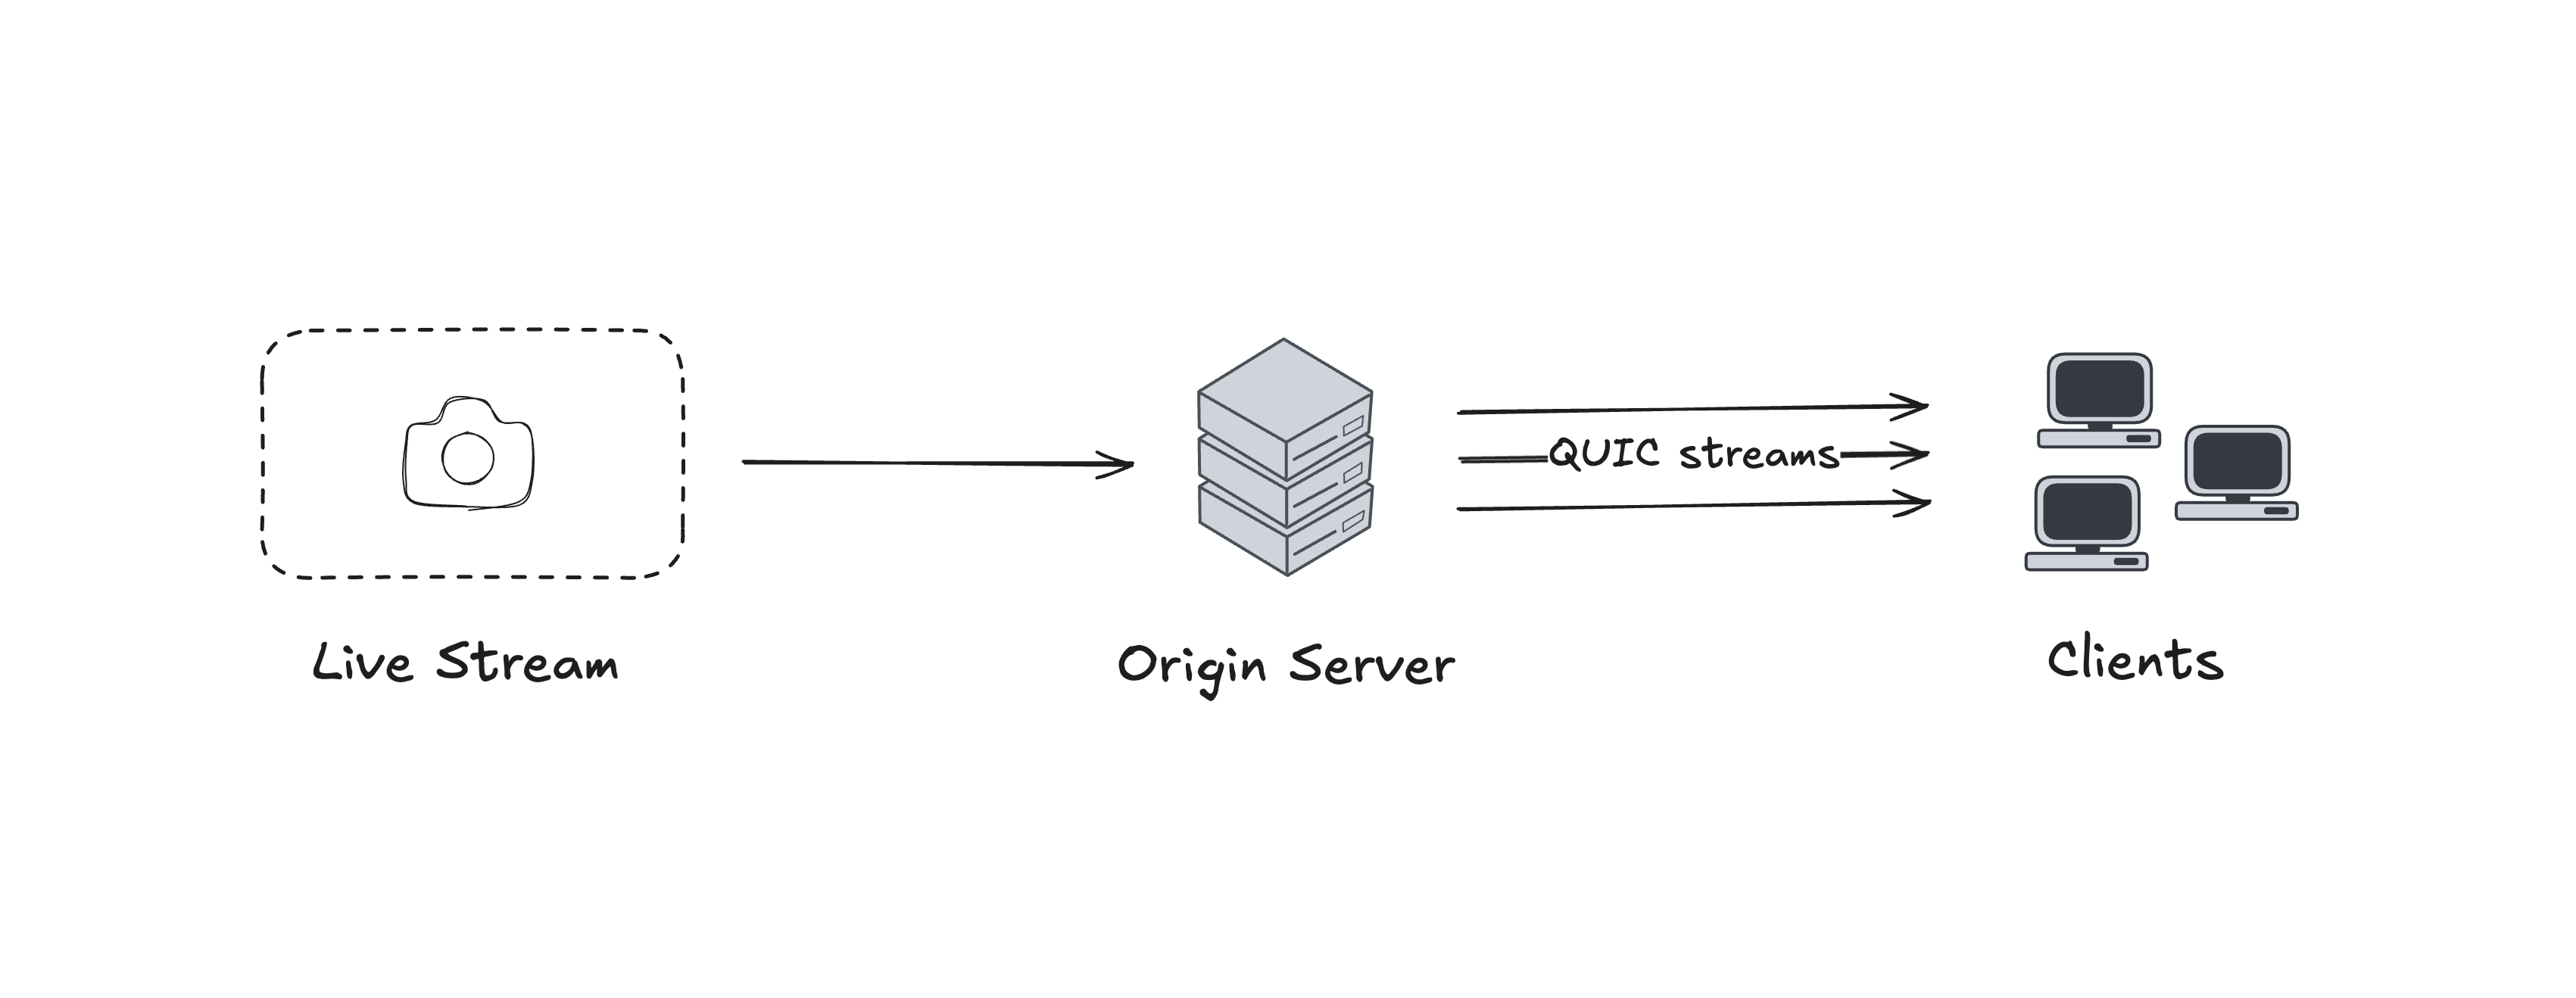
\includegraphics[width=\textwidth]{figures/architecture.png}
    \caption{Architecture of our prototype system}
    \label{fig:architecture}
\end{figure}

\section{Origin server}
The origin server serves a single broadcast. It uses two \ac{MoQ} tracks for this purpose: the \textit{init} track and the \textit{video} track. The init track is used to transmit the ftyp and moov boxes to clients, which contain the information that the client needs to parse the MP4 fragments and decode the video frames. Similar to how clients in a \ac{HAS} system fetch the manifest file, clients subscribe to the init track on startup. The video track is used to serve the actual video content.

The origin server is implemented in Rust and uses moq-transport\footnote{\url{https://crates.io/crates/moq-transport}}, a Rust crate that implements the \ac{MOQT} protocol. The server ingests and broadcasts the stream as follows. First, the server creates a \lstinline{Track} for the init and video tracks. A \lstinline{Track} is an abstraction provided by moq-transport to fan out MoQ objects to multiple subscriptions. Using the \lstinline{Track} API, an application writes objects to the track using a writer handle, and moq-transport notifies any readers reading the track using the reader handles. After creating the tracks, the server starts and executes two processes concurrently.

The server reads the video stream from standard input (stdin), parses the MP4 boxes and writes them to the respective \lstinline{Track}. First, the ftyp and moov boxes are ingested. The server writes a MoQ object containing both boxes to the init track. Following the ftyp and moov boxes is a stream of moof and mdat boxes, with each pair corresponding to an MP4 fragment. The MP4 stream is fragmented at every frame with the FFmpeg option \lstinline{frag_every_frame}\footnote{\url{https://ffmpeg.org/ffmpeg-formats.html\#Options-6}} so that each MP4 fragment contains a single video frame. If the frame contained in the MP4 fragment is a keyframe, the server creates a new MoQ group. Keyframes always introduce new MoQ groups so that clients can start subscriptions at the latest possible point in time, which is the start of the most recent group. For each fragment that is ingested, using a handle to the current group, the server writes an object to the video \lstinline{Track} with the fragment as the object's payload.

Simultaneously, the origin server listens to new subscription requests and serves existing subscriptions by broadcasting the local \lstinline{Track}. For each subscription request that the server receives, it creates an asynchronous, non-blocking \textit{task}, a form of a lightweight thread in Rust, to serve the init or video track to the client. In this task, the server reads the MoQ objects from the local \lstinline{Track}, which are being written in the ingestion process, and transmits them to the client using the existing QUIC connection. To transmit the MoQ object, the server opens a new QUIC stream or uses an existing one, depending on the media to streams mapping configuration. Our baseline implementation transmits the frames reliably and in order, using a single QUIC stream, similar to a traditional live-streaming system that uses TCP. We explore other ways to map media to streams and prioritize these in sections \ref{chapter:deprioritizing_b_frames} and \ref{chapter:skipping_old_media}.


\section{Live streaming client}\label{section:baseline_client}
% TODO: make sure to explain what the render pipeline is, and mention calculateTimeUntilFrame
We now turn our attention to the client.

Subscribing and playing a live stream works as follows. First, the client downloads the ftyp and moov boxes by subscribing to the init track. These boxes contain metadata about the tracks in the MP4 stream % TODO: such as...
that the client will later need to parse the MP4 fragments and decode the video frames.

To initialize playback, the client subscribes to the video track, indicating the \textit{subscribe location}, which specifies where in the track the subscription should start.  Since the player can't start playback in the middle of a \ac{GoP}, two different subscribe locations are possible. The client can wait for the new \ac{GoP} to be produced by using the mode \lstinline{RelativeNext} and the value \lstinline{0}, or it can subscribe to the latest \ac{GoP} with the mode \lstinline{RelativePrevious} and the value \lstinline{0}. On the one hand, waiting for a new GoP to start ensures the lowest possible latency. On the other hand, starting playback at the latest GoP keeps startup delays low but it can lead to latencies up to the duration of a GoP. % TODO: this is not really true, because we can simply subscribe to the latest gop and flush all frames until the last frame or something like this
Whether to prioritize startup delay or latency should be decided based on the use case.

As the client receives the MP4 fragments from the video track, it adds them to a pipeline that processes the raw fragments, extracting the video frames and eventually rendering them. The pipeline consists of three stages. 

First, the player extracts the frame payload and the frame metadata, such as the frame duration, decode timestamp, and presentation timestamp, from the MP4 fragment. 

Then, it decodes the encoded frame with the frame metadata using the VideoDecoder from the WebCodecs API. We configure the decoder using the ftyp and moov boxes, which we downloaded from the init track. To configure the VideoDecoder, two options are worth mentioning. We enable \lstinline{optimizeForLatency} % TODO: What does optimizeForLatency actually do
and set \lstinline{hardwareAcceleration} to \lstinline{"prefer-software"}. We used the latter setting because the VideoDecoder occasionally threw decoding errors on our test machine when hardware acceleration was enabled. % TODO: Elaborate. E.g. These errors could be caused by A deeper issue with our implementation could We are not sure if this is an issue with our implementation or an issue with the WebCodecs API.

Finally, the client renders the decoded frame by drawing it to a canvas element. Rather than rendering the frames directly, we buffer and time the rendering of frames to handle packet jitter, or small variations in the delay of received packets. This ensures that frames are rendered at regular intervals, resulting in smoother playback. After decoding a frame, the player adds it to the buffer. Once the buffer reaches a target size, the player starts consuming frames by retrieving the frame with the lowest timestamp from the buffer and waiting for the correct time to render it. If the buffer runs out of frames, the player stops retrieving frames and waits until the buffer reaches the target size again.

% TODO: explain the algorithm. Explain that resumedPlayingAt is set to undefined when the player first starts, or rebuffers, and that it's set when the first frame is rendered after a pause, or rebuffer event
Algorithm \ref{alg:time_until_frame} shows how the player calculates the time until a frame is to be rendered. The time the player should wait depends on the current media time, which is the elapsed time since playback started in the current session. If the stream can be played without interruptions, the time until a frame is to be rendered is the difference between the frame timestamp and the media time. However, if the player rebuffers, using the absolute media time would cause all frames that are lagging behind to be rendered immediately after the player resumes playback. If the network conditions that led to the rebuffering event are not short-lived, then the player would continuously flush all frames, emptying the buffer, and start buffering again. We handle this issue by timing the rendering of frames relative to the point in time at which playback resumed after a rebuffering event rather than the absolute playback start.  % TODO: However if we do this, it increases latency. Further work needs to be done on this. Find a hybrid strategy

% TODO: Explain that latency keeps increasing if we do this. 
% TODO: Explain that when network recovers and we get a bunch of media we can skip old media by checking if the buffer did grow past a threshold

\begin{algorithm}
\caption{Calculate time to render frame}\label{alg:time_until_frame}
\begin{algorithmic}
\Function{calculateTimeUntilFrame}{$frameTimestamp$}
    \State $now \gets \Call{now}{\null}$
    \item[]
    \If{$resumedPlayingAt = undefined$}
        \State $resumedPlayingAt \gets \textnormal{\{\}}$
        \State $resumedPlayingAt.localTime \gets now$
        \State $resumedPlayingAt.mediaTime \gets frameTimestamp$
    \EndIf
    \item[]
    \State $relativeMediaTime \gets now - resumedPlayingAt.localTime$
    \State $relativeFrameTimestamp \gets \newline
 \hspace*{3em}(frameTimestamp - resumedPlayingAt.mediaTime) / 1000$
    \State \Return $\max(0, relativeFrameTimestamp - relativeMediaTime)$
\EndFunction
\end{algorithmic}
\end{algorithm}


\section{Deprioritizing B-frames}\label{chapter:deprioritizing_b_frames}
% TODO: Make point about this approach making a sense for when the network bandwidth drops slightly below the stream's bitrate
In order to prevent the latency from increasing during network congestion, the server needs to send less data to the client. One way to reduce the stream's bitrate is by dropping B-frames. The reason this works is twofold. 

First, B-frames are not usually depended by other frames, and therefore, they can be dropped without affecting the decodability of other frames. We will assume for the remainder of this section that B-frames are not used as references. We note, however, that state-of-the-art encoders allow the use of B-frames as references through B-pyramid schemes. We will discuss the use of reference B-frames, including ways to adapt our implementation to support them, towards the end of the section. % TODO: Can B-frames be used in low-latency livestreaming

% TODO: make a point about series of snapshots instead of continued video
Second, the I- and P-frames alone form themselves a stream that is playable, albeit with video artifacts, such that we can drop all B-frames if necessary. This is only true if the number of consecutive B-frames is limited, which is the case in low-latency live streaming. % TODO: explain why: since dropping too many frames in a row would result in an incoherent video. If this were not the case, then it would be like we were skipping media. This is a viable strategy, but it's one that requires different ways to render the frames in the client. We will talk about this in the next section.

We effectively divide the stream into two layers: a base layer, consisting of the I- and P-frames, and an enhancement layer containing all B-frames. During congestion, the server drops the enhancement layer, degrading the stream quality to reduce the stream's bitrate.

We prioritize the layers such that the B-frames are sent on a best-effort basis, as follows. The base layer is assigned the highest priority so that the server always transmits I-frames and P-frames, if any are available, first. On the other hand, B-frames are given a lower priority so that they are transmitted only when there is enough network bandwidth.

To implement this, we divide the stream into two MoQ tracks, one for each layer. In both tracks, each GoP forms a group. The group boundaries must be aligned in this way to provide a join point for new subscriptions that is synchronized across both tracks. At startup, the client subscribes concurrently to both tracks referencing the same MoQ group.

The track that serves the base layer uses a single QUIC stream to deliver the I- and P-frames in order. 
% TODO: mention that we are using quinn-rs and how it implements priorities
We assign the second highest priority to this stream. (The highest priority value is assigned to the
init track).

% TODO: Maybe use an excalidraw sketch to make the explanation more clear
To stream the enhancement layer, one could think of using a single stream with a lower priority. However, this simple prioritization strategy wouldn't have the desired effect. We demonstrate the issue with an example. Suppose that the network was congested, and we didn't transmit any B-frames because there wasn't enough bandwidth. When the network recovers, we want to transmit the new B-frames. However, the old B-frames are transmitted because they were queued first. If the network has just enough bandwidth to send the B-frames of one GoP, we would never get a chance to render the B-frames. They would always be late. The same reasoning applies to a stream per GoP for the B-frames. If the server gets enough bandwidth to transmit some B-frames towards the end of a GoP, we don't want to send the first frames of the GoP since they are useless. 

Each B-frame should have a higher priority than the previous B-frame that was produced. In general, frames in enhancement layers should be prioritized according to the new over old policy since they are always transmitted on a best-effort basis. 

Since, in QUIC, the unit of prioritization is the stream, each B-frame needs to be sent in a separate stream. The decode timestamps of B-frames can be used as the priority for each stream, or if one wants to make optimal use of the number of bits, the current count of B-frames.

% TODO: fix this. a single frame can contains slices of all types
To prioritize I- and P-frames over B-frames, the server must be able to distinguish frames of different types in the first place. Identifying the type of a frame is not as trivial as one might think. Parsing the MP4 fragments is not enough because there don't exist any boxes in the MP4 container that contain this information. One needs to parse the encoded sample. For H.264/AVC encoded frames, for example, we first parse the \ac{NAL} units with the type 0 or 5, which correspond to coded slices of a non-IDR picture and coded slices of an IDR picture respectively, from the MP4 sample. We then parse the slice types from the slice header of these NAL units.

Additionally, the server includes the frame type in the header of the payload of the MoQ object, such that clients, and potentially relays as well, can easily extract the type of a frame from the MoQ object without having to parse the encoded samples.

\subsection{Handling out-of-order frames}\label{section:out_of_order_frames}
% TODO (maybe): instead of explaining why they can arrive out-of-order, simply say that is best to assume they will arrive out-of-order because nothing guarantees that they will arrive in order when we use multiple streams
Because we are using multiple QUIC streams, which are independent and don't provide any ordering guarantees, frames may arrive out-of-order. Within the base layer, I- and P-frames will arrive in decode order. However, B-frames can arrive out-of-order relative to the frames in the base layer. Furthermore, B-frames can arrive out-of-order relative to each other. First, if the network becomes temporarily congested such that some B-frames are not transmitted, then old B-frames will be sent to the client when the network recovers. Second, a B-frame can arrive ahead of another B-frame that was sent first because the underlying packets take different network paths or due to packet loss. % TODO: cite source
In this subsection, we propose a solution to this issue. First, we explain the intuition behind our approach, and then we describe it more precisely by explaining relevant implementation details.

% TODO: explain what the render pipeline is (in the baseline version section)
We add frames from the base layer, which arrive in order relative to each other directly to the render pipeline. Although there might be discontinuities between these frames, we don't wait for the missing B-frames because they might never arrive.

B-frames can be late or early. We define a B-frame to be late if, at the time of its arrival, a frame with a higher timestamp has already arrived. Similarly, we say a B-frame is early if it arrives ahead of frames with a lower timestamp. If a B-frame is late, we drop it because we don't want to decode and render frames out-of-order. If a B-frame is early and no later I- or P-frames have arrived, we wait for the earlier frames to arrive. This is because the B-frame might have arrived ahead of a frame from the base layer, which we can't drop. Note that the B-frame might simply be ahead of other B-frames, but we have no way of telling, so we need to assume the worst case. If a B-frame is neither late nor early by our definitions, we add it directly to the render pipeline. 

\begin{algorithm}
    \caption{Reorder Algorithm}\label{alg:reorder}
    \begin{algorithmic}
    \Function{reorder}{$frame$}
        \If{$frame.type = B \land lastEnqueued \neq null \land frame.dts < lastEnqueued.dts$}
            \State \Return \Comment{Drop late B-frames}
        \EndIf
        \item[]
        \State add $frame$ to $buffer$
        \item[]
        \While{$\Call{bufferSize}{\null} > targetSize$}
            \State $next \gets buffer[0]$
            \If{\newline
                \hspace*{4.5em}$next.type \neq B \lor \newline
 \hspace*{4.5em}lastEnqueued = null \lor \newline
 \hspace*{4.5em}next.dts = lastEnqueued.dts + lastEnqueued.duration$\newline\hspace*{2.7em}}
                \State enqueue $next$
                \State pop $buffer$
                \State $lastEnqueued \gets next$
                \State \textbf{continue}
            \EndIf
            \item[]
            \State $i \gets 1$ \Comment{B-frame is early}
            \While{$i < buffer.length \land buffer[i].frameType = B$}
                \State $i \gets i + 1$
            \EndWhile
            \If{$i < buffer.length$} \Comment{B-frame is not ahead of any I-, or P-frames}
                \State enqueue $next$
                \State pop $buffer$
                \State $lastEnqueued \gets next$
            \Else \Comment{Wait, because B-frame might be ahead of I-, or P-frames}
                \State \textbf{break} 
            \EndIf
        \EndWhile
    \EndFunction
    % \item[]
    % \Function{bufferSize}{\null}
    %     \If{$buffer.length = 0$}
    %         \State \Return 0
    %     \EndIf
    %     \item[]
    %     \State $oldest \gets buffer[0]$
    %     \State $newest \gets buffer[buffer.length - 1]$
    %     \State \Return $newest.dts - oldest.dts$
    % \EndFunction
    \end{algorithmic}
\end{algorithm}

In practice, frames that are in order are not added directly to the render pipeline. Instead, frames are first added to a buffer to handle small variations in the arrival of frames. Otherwise, if we add frames directly to the render pipeline, a frame that is late by only a few milliseconds will be dropped. From our experiments, we found a 100 to 200 milliseconds buffer to be optimal. % optimal in what sense? explain

% TODO: double check correctness of the algorithm and reasoning
% TODO: explain that buffer works like a priority queue, and buffer[0] is the frame with the lowest decode timestamp and buffer[buffer.length - 1] is the frame with the highest timestamp
% Explain the bufferSize function?
% explain why you use a while loop instead of an if statement
Algorithm \ref{alg:reorder} shows pseudocode for the process of handling an incoming frame and retrieving the next frame to be enqueued to the render pipeline. First, we check if the frame is a B-frame and if the frame is late by checking if it has a lower decode timestamp than the decode timestamp of the last enqueued frame. If the B-frame is late, we drop it. Otherwise, we add the frame to the buffer. This buffer works like a min-heap, with the decode timestamps (DTS) serving as the key. Then, if the buffer size is greater than the target size, we \textit{try} to retrieve the next frames from the buffer and enqueue them to the render pipeline. To do this, we check the frame with the lowest timestamp in the buffer. If the frame is an I- or P-frame or if there are no discontinuities between the frame's DTS and the DTS of the last enqueued frame, we enqueue the frame to the buffer and try to enqueue the next frame. If the frame is a B-frame and it is early, then we scan the buffer for an I- or P-frame. If we find an I- or P-frame, then it must be the case that the frame has a higher timestamp, and we enqueue the frame. Note that the B-frame cannot be ahead of any I- or P-frames since frames from the base layer are transmitted in order. If, on the other hand, the buffer only has B-frames, then we wait for the missing frames to arrive by returning since it might be ahead of I- or P-frames.

\subsection{Reference B-frames}\label{section:reference_b_frames}
We assumed until now that B-frames are not depended on by other frames. However, H.264 and newer video codings allow B-frames to be used as references for the encoding of other frames. Dropping a B-frame that is used as a reference while trying to decode the dependent frames will cause video distortions. A decoder can't decode a frame without its dependencies without errors. The approach we described so far doesn't distinguish between reference and non-reference B-frames, and therefore, video distortions will occur when the network is congested.

The simplest solution is to disable the use of B-frames as references, at the cost of a slightly lower coding efficiency. For H.264/AVC, one can control this with the b-pyramid setting\footnote{\url{https://en.wikibooks.org/wiki/MeGUI/x264\_Settings\#b-pyramid}}. In live streaming, the decrease in coding efficiency resulting from disabling this option is limited since we use a relatively low number of B-frames.

However, one might not be able to configure the encoder settings. A production live streaming platform, for example, might ingest streams from a variety of sources, of which the user is in control of the encoding configuration. In these cases, one must design a streaming protocol that handles reference B-frames properly.

One approach consists of distinguishing reference from non-reference B-frames and transmitting reference B-frames together with the I- and P-frames. In the client, we wait for any reference B-frames if a non-reference B-frame arrives early, just like we do for I- and P-frames. This ensures that reference B-frames are not dropped, and therefore, we don't cause video distortions. To identify the reference B-frames, one can try using the MP4 sample flags \lstinline{sample_depends_on} and \lstinline{sample_is_depended_on}. % TODO: cite mp4 spec
We note, however, that in our experiments, both flags were set to the value $0$, indicating that the dependencies were unknown for the majority of frames. One can also try identifying reference B-frames by parsing the \ac{NAL} units of the H.264/AVC encoded stream. 

We propose a different approach that doesn't require knowing precisely which B-frames are used as references. This approach is based on the observation that B-frames with a lower decode order are more likely to be referenced by other B-frames. Recall that whenever a frame depends on a future frame, which is the case with B-frames or bi-directional predicted frames, the future frame is encoded first and, therefore, has a lower decode timestamp. Frames only depend on frames with a lower decode order. 

\begin{figure}
    \centering
    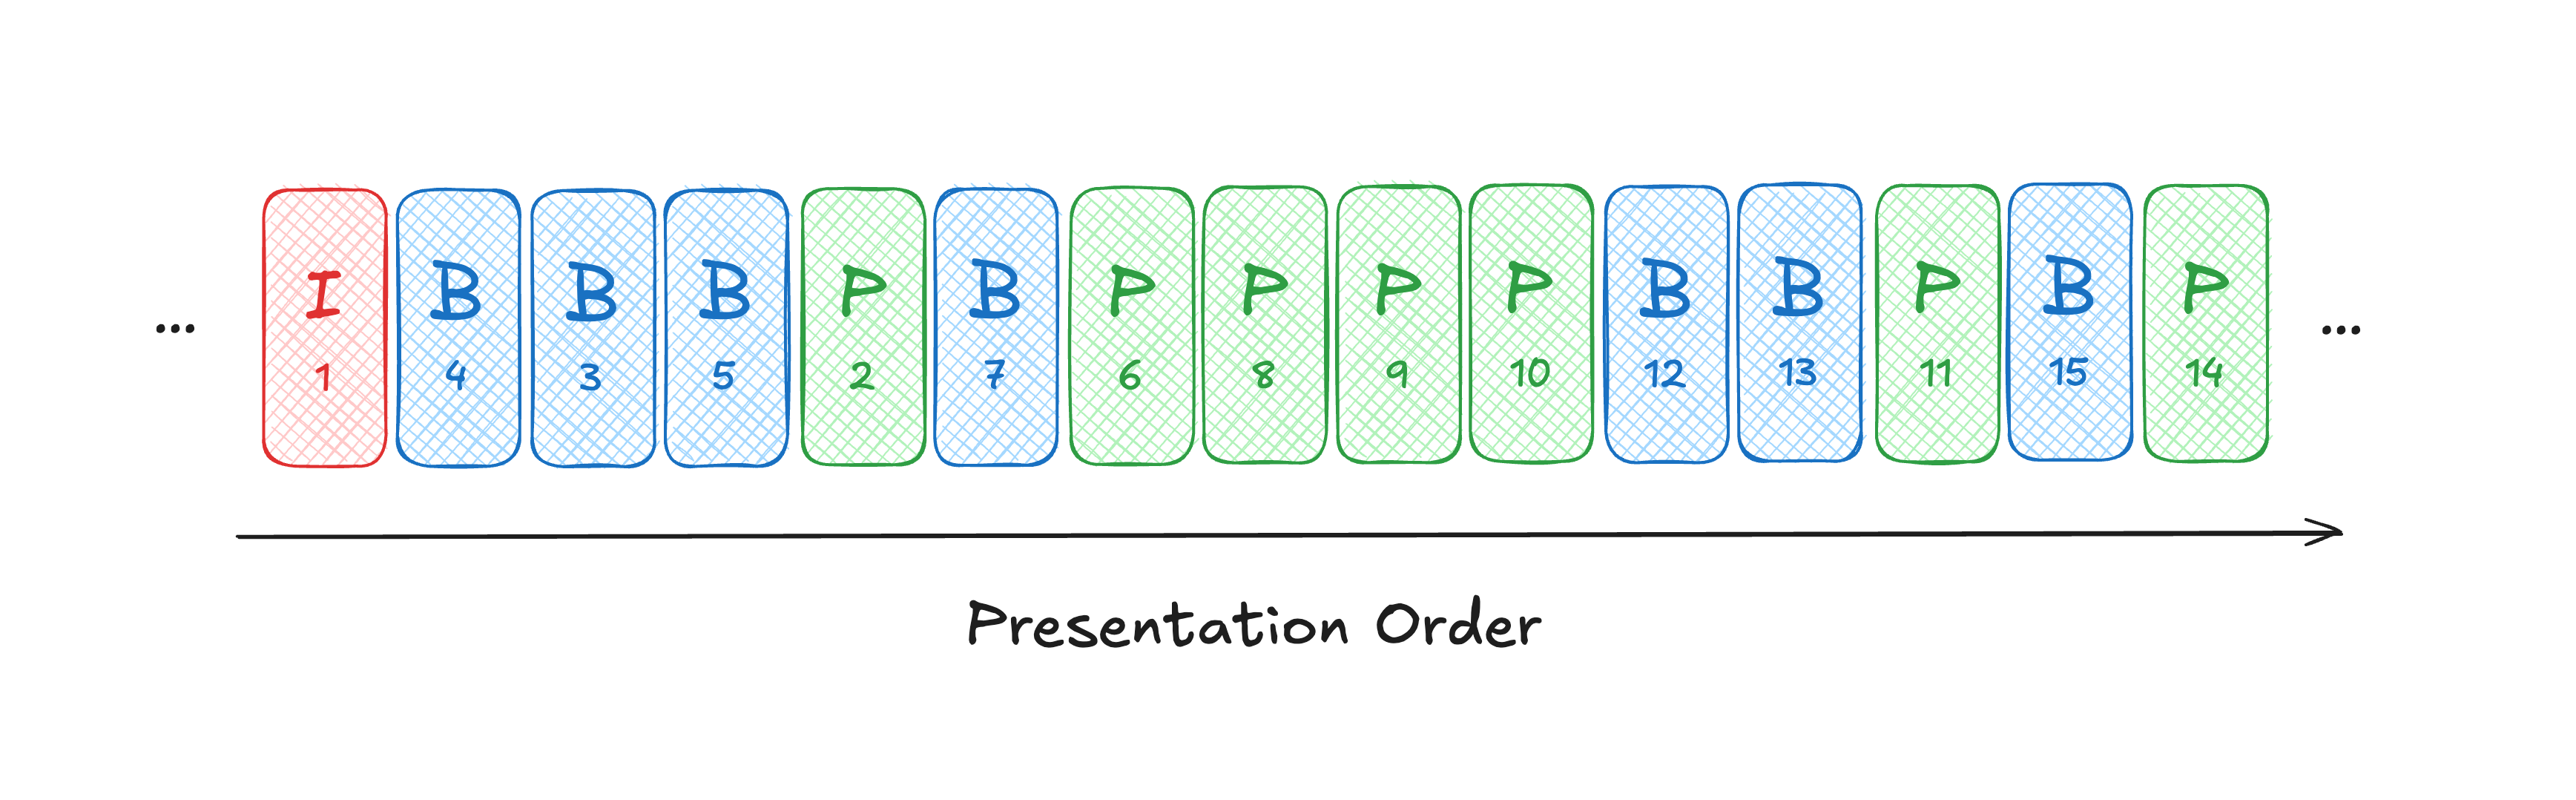
\includegraphics[width=\textwidth]{figures/gop_structure.png}
    \caption{Example \ac{GoP} with frames and their decode order}
    \label{fig:gop_structure}
\end{figure}

We found this heuristic to work well for \ac{GoP} structures with a maximum of three B-frames between each I-  or P-frame. We haven't tested \ac{GoP} structures that use more than three B-frames since using more than three B-frames is not common in low-latency live streaming. From our experiments, we observed that when there were consecutive B-frames, the first two frames were always out of order, as we can see in the first group of B-frames in \autoref{fig:gop_structure}. This indicates that the second B-frame is being used as a reference by the first B-frame, otherwise the two frames wouldn't be out of order. Furthermore, dropping only the second B-frame caused very noticeable video distortions, both for the first and third frames in the group, as shown in \autoref{fig:video_artifacts}. We conclude that in addition to the first B-frame, the third B-frame also depends on the second B-frame. On the other hand, dropping the second and third B-frames didn't cause any video distortions, and therefore, we assume that these frames are not used as references. With less than three consecutive B-frames, none was used as a reference in our experiments.

% Recall that B-frames, bi-directional predicted frames, reference both a preceding frame and a future frame. For this reason, future frames that are depended by B-frames come before than the B-frames that reference it. 

\begin{figure}
    \centering
    \begin{subfigure}{\textwidth}
        \centering
        
\includegraphics[width=0.3\textwidth]{figures/video_artifacts/all_frames/frame_00167.png}
        
\includegraphics[width=0.3\textwidth]{figures/video_artifacts/all_frames/frame_00168.png}
        
\includegraphics[width=0.3\textwidth]{figures/video_artifacts/all_frames/frame_00169.png}
        \caption{Original frames}
    \end{subfigure}

    \vspace{1em}

    \begin{subfigure}{\textwidth}
        \centering
        
\includegraphics[width=0.3\textwidth]{figures/video_artifacts/drop_first_b_frame/frame_00149.png}
        
\includegraphics[width=0.3\textwidth]{figures/video_artifacts/drop_first_b_frame/dropped.png}
        
\includegraphics[width=0.3\textwidth]{figures/video_artifacts/drop_first_b_frame/frame_00150.png}
        \caption{Frames decoded without the second B-frame}
    \end{subfigure}
    \caption{Video artifacts caused by dropping the second B-frame of a group of three consecutive B-frames}
    \label{fig:video_artifacts}
\end{figure}

Since B-frames with a lower decode order are more likely to be used as references, we prioritize older B-frames over newer ones within a group of consecutive B-frames so that frames that are depended on are more likely to be delivered first. We will use the term B-frame group to denote a group of consecutive B-frames. Across B-frame groups, we use the same new over old policy by assigning a higher priority to newer groups. Note, however, that H.264/AVC allows P-frames to reference B-frames. As a result, video distortions will still occur whenever a B-frame that is referenced by a P-frame is dropped.

% An alternative is to transmit reference B-frames with a lower priority than I-, and P-frames, but with a higher priority than non-reference B-frames. This is a sensible approach, particularly when the encoder uses a \ac{GoP} structure, in which reference B-frames are only referenced by other B-frames. To minimize video distortions, we still drop non-reference B-frames if the   Furthermore, we drop non-reference B-frames if the respective reference B-frame hasn't arrived. This is based on the observation that skipping the rendering of the other B-frames has a much less noticeable impact on video quality than rendering the two B-frames with video distortions.


% The  The drawback is that we can't fully eradicate video distortions, since P-frames can also reference B-frames. However, only a few P-frames reference B-frames and the impact of dropping the reference B-frame is much smaller, because they reference much less macroblocks of the B-frame, and therefore the impact on the frame is much lower, as shown in the P-frame in \autoref{fig:video_artifacts}. 

% We implement this priority scheme as follows. Let $P_k \in [0, P_{max}]$ be the priority of frame $k$. $P_k$ can be formulated as:

% \begin{align*}
%     P_k &= P_{max}, & \text{if } k \text{ is an I-, or P-frame} \\
%     P_k &= (G_k \ll b) + 2^b - I_k, & \text{if } k \text{ is a B-frame}\\
% \end{align*}

\section{Skipping old GoPs}\label{chapter:skipping_old_media}
Degrading the stream quality by deprioritizing B-frames is one way to decrease latency when the network is congested, but it is not enough to handle large changes in the network bandwidth. Consider the case where a viewer is watching a live stream on their phone, and the available network bandwidth drops drastically and then recovers. This can happen because the viewer is watching the live stream on his phone while on the move and temporarily passes through an area with poor coverage, for example. While the network connectivity is poor, streaming a lower quality stream surely helps. However, video will still lag behind, and latency will increase due to the low network throughput. Video will queue at the server. When the network recovers, rather than playing all the video that is queued, we want to resume playback at the live edge. We want to skip large portions of media if we don't get a chance to transmit it due to network conditions.

% TODO: mention Warp
To achieve this, we prioritize new over old media. Specifically, we map and prioritize the video track as follows. We map each GoP of the video stream to a MoQ group and send each group in its own QUIC stream. We prioritize new GoPs over old ones by using the timestamp of the first frame in the group as the priority of the QUIC stream.

% In the client, we drop any frames belonging to old GoPs. Handling late GoPs is similar to how we handled out-of-order frames in \autoref{section:out_of_order_frames}. One can keep track of the last frame that we enqueued to the processing pipeline and compare the timestamps of new frames with the timestamp of this frame, dropping the new frames if they have a lower timestamp. % TODO: Note that as opposed to subsection 2.2.2, we don't use a jitter buffer, because it doesn't make sense % TODO: Explain why

\subsection{Snapping video forward}\label{section:snapping_video_forward}
% TODO: Explain what i mean with jumping playback more clearly
Our goal is to render new media immediately, such that playback jumps from the old media forward to the new media. Recall, however, that the player, as we first described in \autoref{section:baseline_client}, times the rendering of frames using the relative frame timestamp. Using Algorithm \ref{alg:time_until_frame} to time the rendering of new media would result in the player waiting for the frame's timestamp before rendering the new GoPs, and thereby not decreasing the latency. On the one hand, we want to render new media immediately. On the other hand, we want to buffer and time consecutive frames according to their presentation time for smoother playback. To achieve this, we compare the presentation timestamp of the previously rendered frame and the frame that we are about to render. If there is a discontinuity between the presentation timestamps, we render the frame immediately; otherwise, we time the rendering of the frame.

To implement this, the client keeps track of the timestamp of the last frame that was rendered, and we adapt Algorithm \ref{alg:time_until_frame} so that it first checks if there is a discontinuity between $frameTimestamp$ and the timestamp of the last rendered frame. If there is a discontinuity, $calculateTimeUntilFrame$ returns 0 so that the frame is rendered immediately. Note that if there is a discontinuity, we also need to update $resumedPlayingAt$ so that we use the correct media time as the reference when timing the next frames.

% Regarding the client, we use the approach described in \autoref{section:snapping_video_forward} with a small modification. Rather than rendering frames instantly if there is any discontinuity, we time frames if the discontinuity is bigger than a predefined threshold. This is because frames from the base layer might have discontinuities, if we drop B-frames, and we don't want to render them immediately. % TODO: Expand on this. The question is what's the threshold? When are two frames too far apart, such that we should render the later frame instantly. % TODO: Finish this part

% TODO: Find a better name
\section{Combining both strategies}
Ideally, we want the live streaming system to handle both small prolonged drops in the network bandwidth and short spikes effectively. While we have not yet confirmed our hypothesis, we believe that skipping old \acp{GoP}, while also deprioritizing B-frames, would result in the most optimal \ac{QoE}. In this section, we propose an approach that combines the two strategies.

We divide the broadcast into two \ac{MoQ} tracks, a track for the base layer that consists of the I- and P-frames and a track for the B-frames, which form the enhancement layer, like we did in \autoref{chapter:deprioritizing_b_frames}. However, rather than using a stream per track, we use a stream per \ac{GoP} for the base layer like in \autoref{chapter:skipping_old_media}. Each B-frame is transmitted in its own stream.

To prioritize the QUIC streams, the idea is to prioritize new over old media and frames from the base layer over frames from the enhancement layer. The latest \ac{GoP} in the base layer is given the highest priority, followed by the B-frames from the latest \ac{GoP}, such that they are transmitted next if there is sufficient network bandwidth. Old \acp{GoP} have lower priorities.

% In the client, we handle frames in the same way as described in \autoref{section:snapping_video_forward}.

% TODO: Give a back-of-the-envelope calculation type of example
An important caveat is that this priority scheme requires many priority values, one for each \ac{GoP} and each B-frame, and it is possible that there aren't enough to cover the entire live stream. quinn-rs\footnote{\url{https://github.com/quinn-rs/quinn}}, for example, which is the QUIC implementation used by moq-rs, uses 32 bits to represent the priority value, which might not be sufficient if the \acp{GoP} are short, and the frame rate of the video stream is high. One can address this issue, by wrapping the priority values around when the maximum value is exceeded. However, if any streams are queued when this occurs, then these streams will have a higher priority than the new streams. The client can close the old streams immediately upon receiving them, but the server will always transmit at least some bytes of the old streams and will keep transmitting them until it receives the \lstinline{STOP_SENDING} QUIC frame. Furthermore, the new streams won't start to be transmitted until this process occurs for all old streams. So far, we haven't been able to identify a solution, and further work is needed to resolve this issue.